\documentclass{article}
\input{../../../../../../LaTex/preamble/preamble_article.tex}

\begin{comment}
    水平双图
    \begin{figure}[h]
    \begin{minipage}{0.45\textwidth}
        \centering
        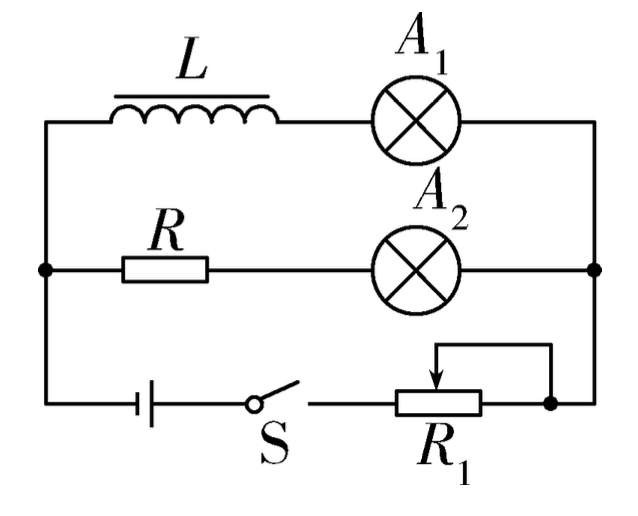
\includegraphics[width = \textwidth]{pictures/1.png}
        \caption*{Figure 1 $L$很大但无铁芯}
    \end{minipage}
    \hfill
    \begin{minipage}{0.43\textwidth}
        \centering
        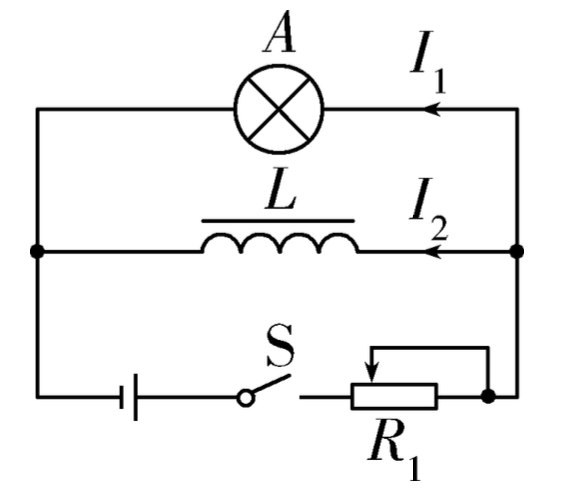
\includegraphics[width = \textwidth]{pictures/2.png}
        \caption*{Figure 2 $L$很大且有铁芯}
    \end{minipage}
    \end{figure}
   

\end{comment}


\title{电磁感应 \quad 单杆模型}
\author{马祥芸}

\begin{document}
\maketitle
\tableofcontents
\newpage
\zihao{-4}



\section{电感在电路中的表现}
\subsection{通电自感与断电自感}
\begin{itemize}
    \item 自感电动势: $ E = L \frac{\triangle I}{\triangle t } $
    \item 自感系数影响因素: 线圈大小,形状,匝数以及是否有铁芯
\end{itemize}

\begin{figure}[h]
    \begin{minipage}{0.45\textwidth}
        \centering
        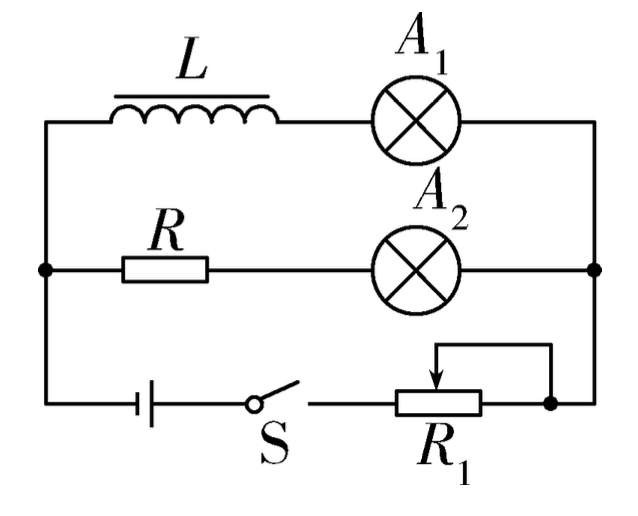
\includegraphics[width = \textwidth]{pictures/1.png}
        \caption*{Figure 1 $L$很大但无铁芯}
    \end{minipage}
    \hfill
    \begin{minipage}{0.43\textwidth}
        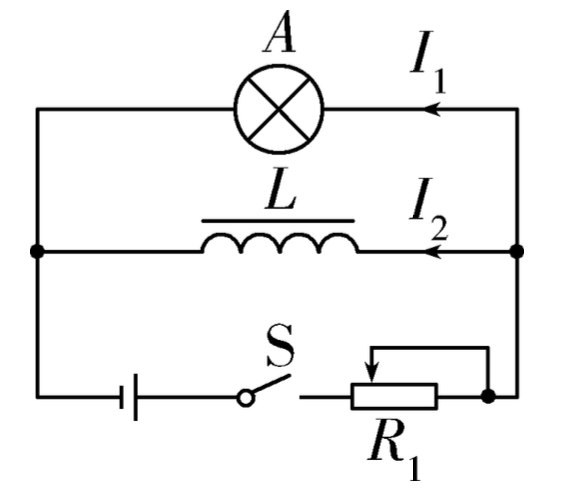
\includegraphics[width = \textwidth]{pictures/2.png}
        \caption*{Figure 2 $L$很大且有铁芯}
    \end{minipage}
\end{figure}

\vspace{2em}

\begin{tabular}{|p{0.2\textwidth}|p{0.4\textwidth}|p{0.4\textwidth}|}
    \hline
    \multicolumn{1}{|c|}{}    &                &                \\
    \multicolumn{1}{|c|}{}    & \hspace{7em}图1 & \hspace{7em}图2 \\
    \multicolumn{1}{|c|}{}    &                &                \\
    \hline

    \multicolumn{1}{|c|}{}    &                &                \\
    \multicolumn{1}{|c|}{}    &                &                \\
    \multicolumn{1}{|c|}{通电时} &                &                \\
    \multicolumn{1}{|c|}{}    &                &                \\
    \multicolumn{1}{|c|}{}    &                &                \\
    \hline
    \multicolumn{1}{|c|}{}    &                &                \\
    \multicolumn{1}{|c|}{}    &                &                \\
    \multicolumn{1}{|c|}{}    &                &                \\
    \multicolumn{1}{|c|}{}    &                &                \\
    \multicolumn{1}{|c|}{}    &                &                \\
    \multicolumn{1}{|c|}{断电时}    &                &                \\
    \multicolumn{1}{|c|}{}    &                &                \\
    \multicolumn{1}{|c|}{}    &                &                \\
    \multicolumn{1}{|c|}{}    &                &                \\
    \multicolumn{1}{|c|}{}    &                &                \\
    \hline
    \multicolumn{1}{|c|}{}    &
    \multicolumn{2}{|c|}{}                                      \\
    \multicolumn{1}{|c|}{总结}  &
    \multicolumn{2}{|c|}{}                                      \\
    \multicolumn{1}{|c|}{}    &
    \multicolumn{2}{|c|}{}                                      \\
    \hline
\end{tabular}

\vspace{2em}

\begin{center}
    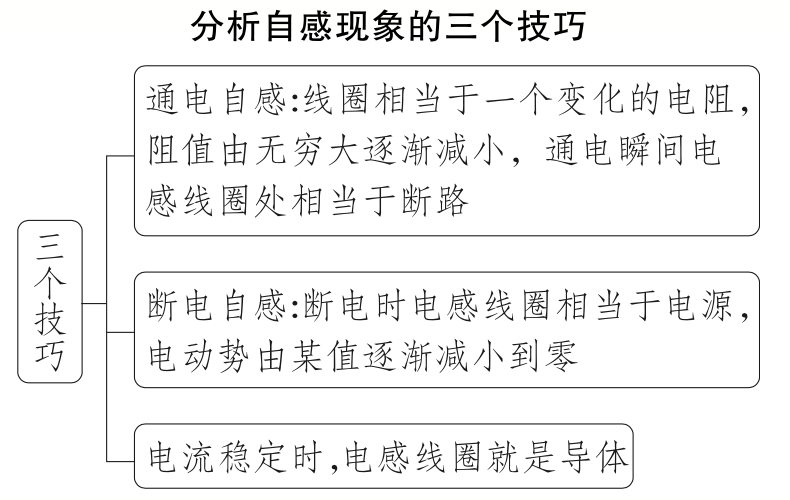
\includegraphics[width = 0.6\textwidth]{pictures/3.png}
\end{center}

\vspace{2em}

\section{单杆模型}

\subsection{单杆电阻类}
\begin{enumerate}[label = (\arabic*{})]
    \item 仅初速度
          \begin{figure}[H]
              \begin{minipage}{0.65\textwidth}
                  \centering
                  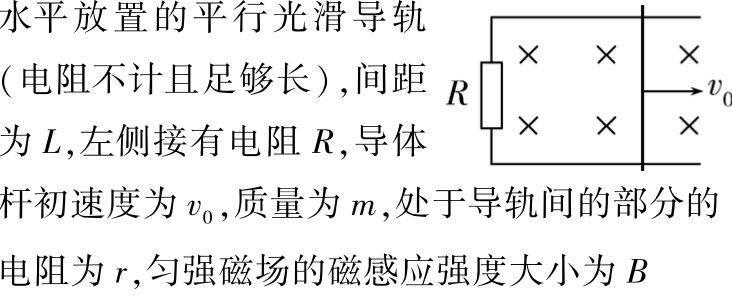
\includegraphics[width = \textwidth]{pictures/4.png}
                  \caption*{Figure 1 情景}
              \end{minipage}
              \hfill
              \begin{minipage}{0.3\textwidth}
                  \centering
                  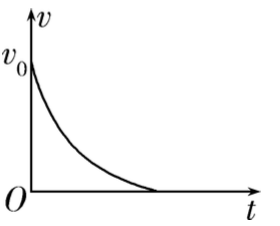
\includegraphics[width = \textwidth]{pictures/5.png}
                  \caption*{Figure 2 运动过程}
              \end{minipage}
          \end{figure}

          \vspace{2em}

          \begin{itemize}
              \item 能量角度:
                    \vspace{5em}
              \item 动量角度:
                    \newpage
              \item 习题

                    \centering
                    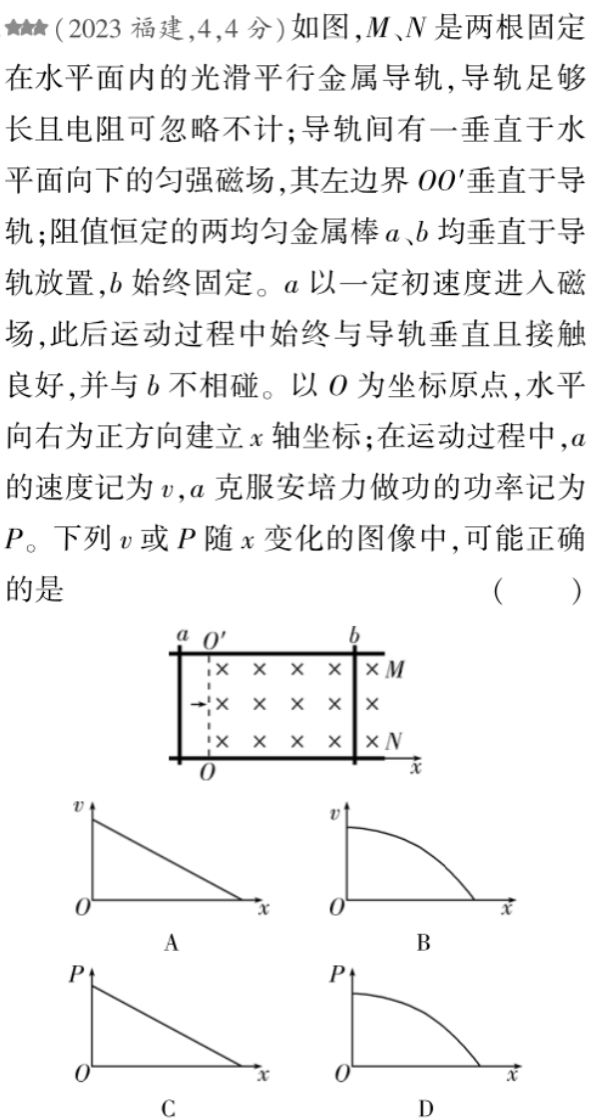
\includegraphics[width = 0.6\textwidth]{./pictures/17.png}

          \end{itemize}

          \newpage

    \item 仅受恒力

          \begin{figure}[H]
              \begin{minipage}{0.6\textwidth}
                  \centering
                  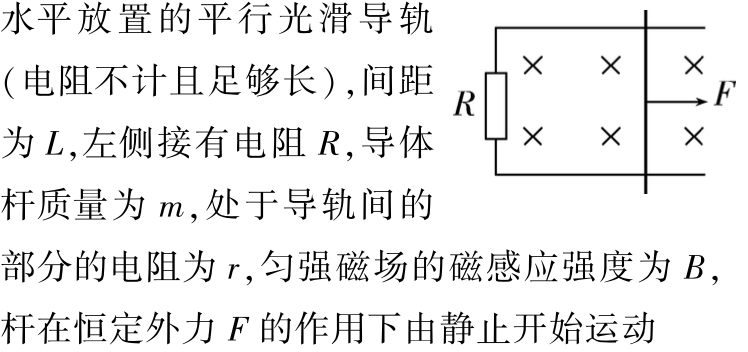
\includegraphics[width = \textwidth]{pictures/6.png}
                  \caption*{Figure 1 情景}
              \end{minipage}
              \hfill
              \begin{minipage}{0.35\textwidth}
                  \centering
                  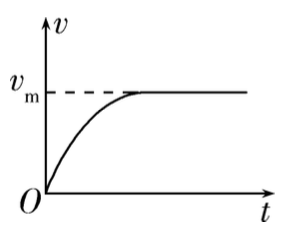
\includegraphics[width = \textwidth]{pictures/7.png}
                  \caption*{Figure 2 运动过程}
              \end{minipage}
          \end{figure}
\end{enumerate}

\vspace{2em}

\begin{itemize}
    \item 能量角度:
          \vspace{5em}
    \item 动量角度:
          \vspace{5em}
    \item 习题

          \centering
          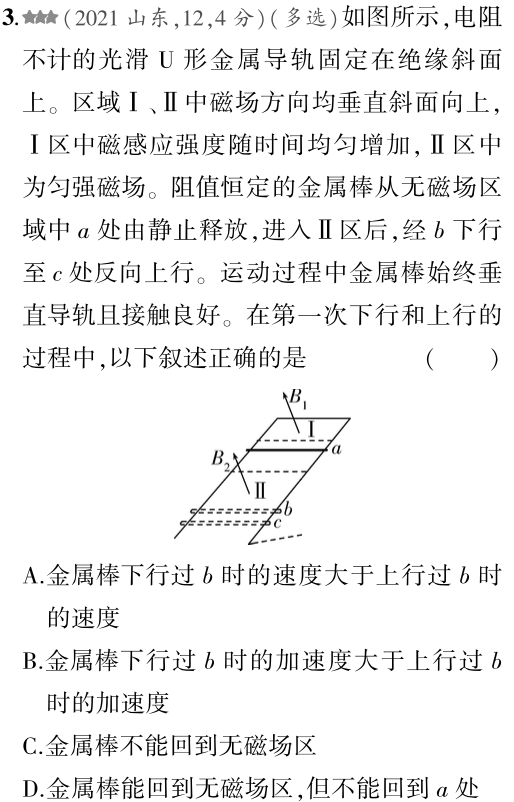
\includegraphics[width = 0.43\textwidth]{./pictures/18.png}

\end{itemize}

\vspace{2em}

\subsection{单杆电源类}

\begin{figure}[H]
    \begin{minipage}{0.65\textwidth}
        \centering
        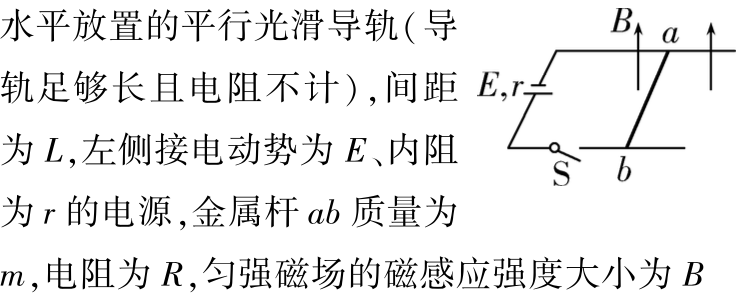
\includegraphics[width = \textwidth]{pictures/8.png}
        \caption*{Figure 1 情景}
    \end{minipage}
    \hfill
    \begin{minipage}{0.3\textwidth}
        \centering
        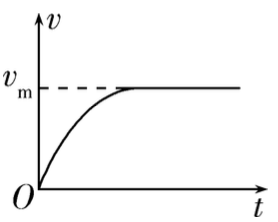
\includegraphics[width = \textwidth]{pictures/9.png}
        \caption*{Figure 2 运动过程}
    \end{minipage}
\end{figure}

\vspace{2em}

\begin{itemize}
    \item 能量角度:
          \vspace{5em}
    \item 动量角度:
          \vspace{5em}
    \item 习题

          \centering
          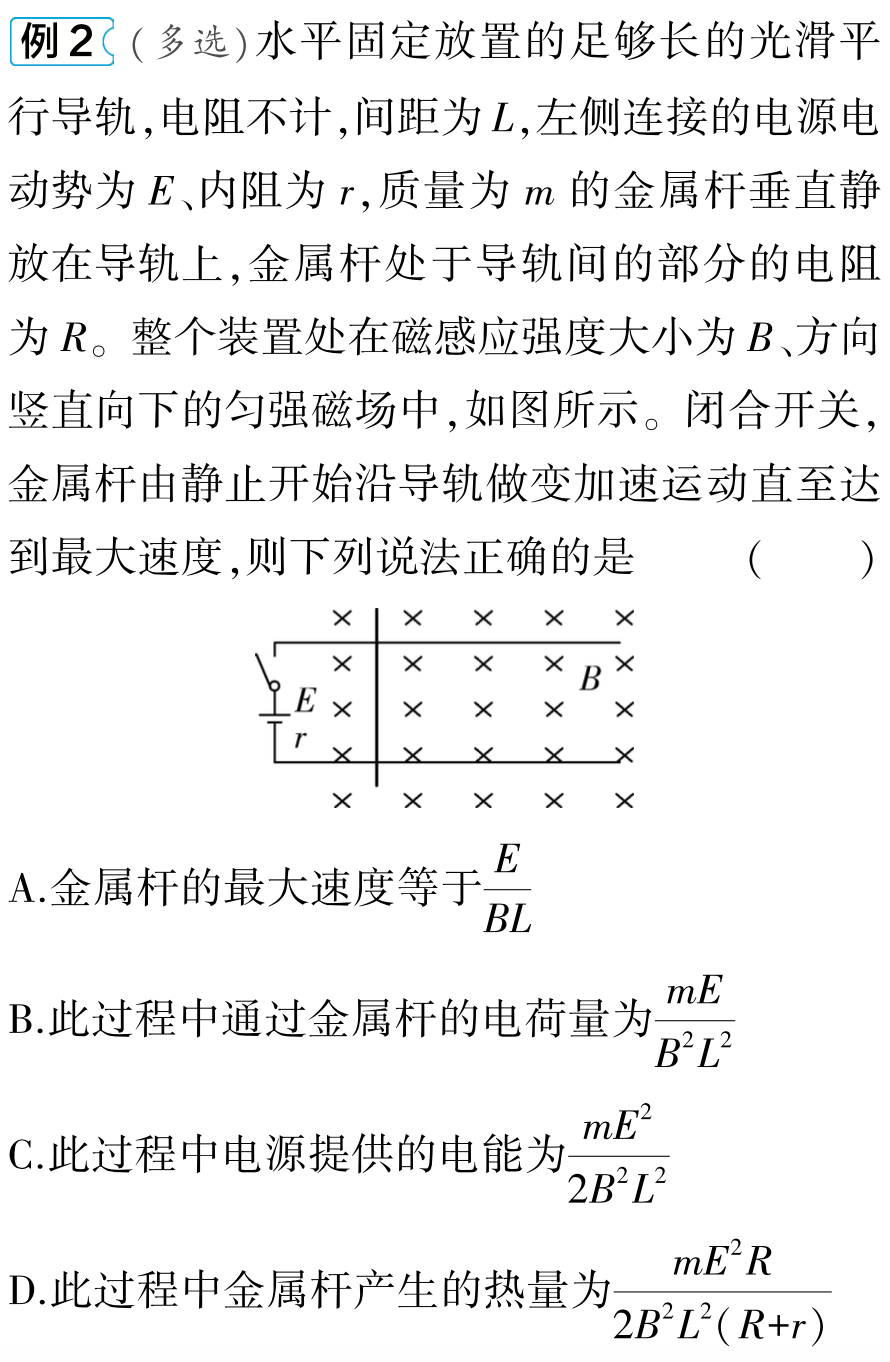
\includegraphics[width = 0.45\textwidth]{./pictures/10.png}

          \vspace{2em}

          \centering
          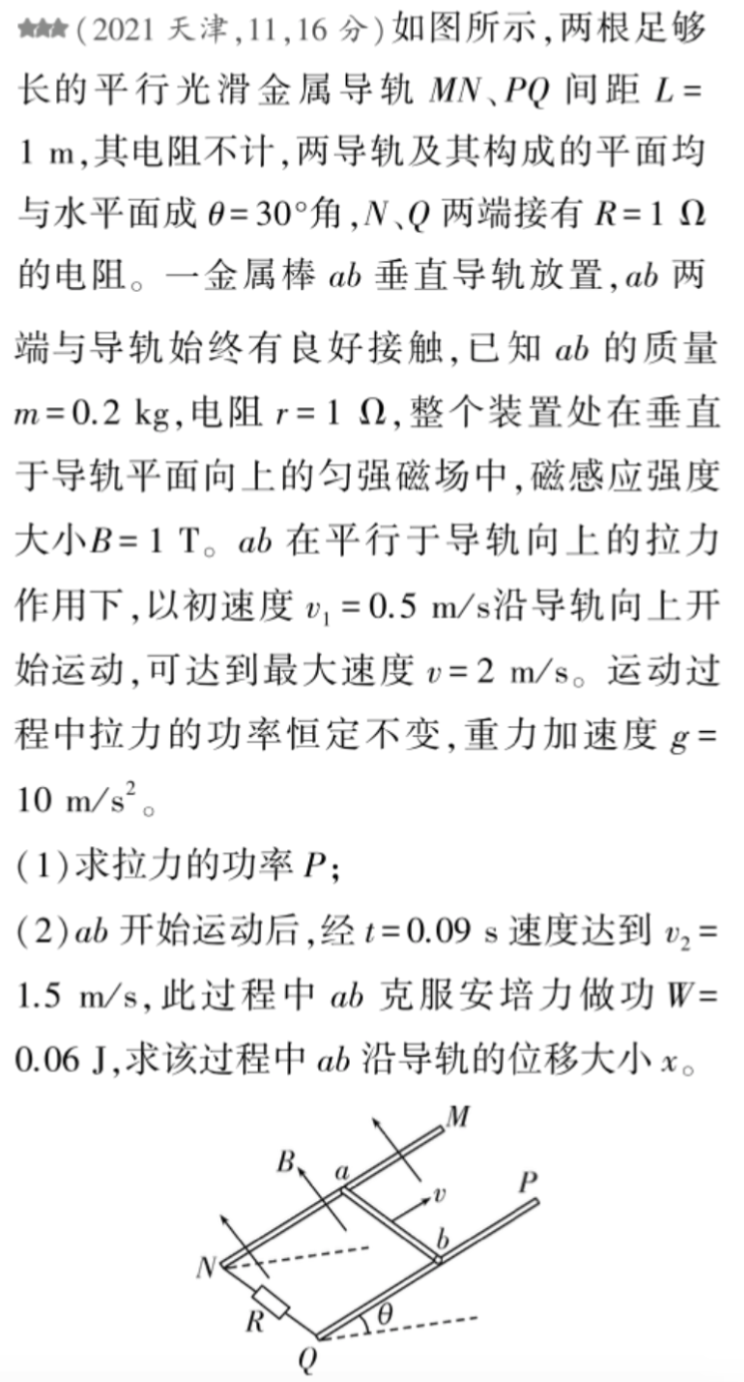
\includegraphics[width = 0.45\textwidth]{./pictures/19.png}


\end{itemize}

\vspace{2em}

\subsection{单杆电容类}
\subsubsection{电容充电式}
\begin{enumerate}[label = (\arabic*{})]
    \item 仅初速度

          \begin{figure}[h]
              \begin{minipage}{0.65\textwidth}
                  \centering
                  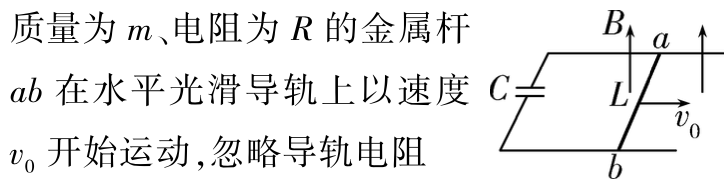
\includegraphics[width = \textwidth]{pictures/11.png}
                  \caption*{Figure 1 情景}
              \end{minipage}
              \hfill
              \begin{minipage}{0.3\textwidth}
                  \centering
                  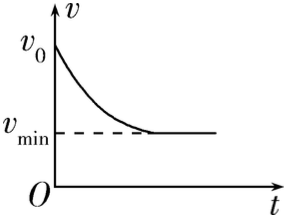
\includegraphics[width = \textwidth]{pictures/12.png}
                  \caption*{Figure 2 运动过程}
              \end{minipage}
          \end{figure}

          \newpage

          \begin{itemize}
              \item 能量角度:
                    \vspace{5em}
              \item 动量角度:
                    \vspace{5em}
          \end{itemize}

          \vspace{2em}

    \item 仅受恒力

          \begin{figure}[H]
              \begin{minipage}{0.7\textwidth}
                  \centering
                  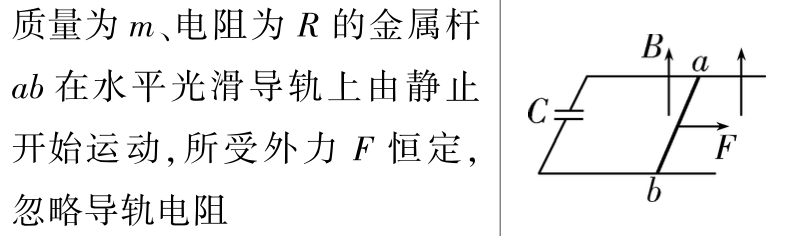
\includegraphics[width = \textwidth]{pictures/13.png}
                  \caption*{Figure 1 情景}
              \end{minipage}
              \hfill
              \begin{minipage}{0.25\textwidth}
                  \centering
                  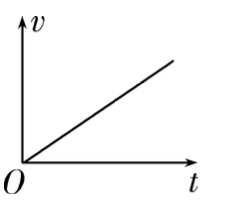
\includegraphics[width = \textwidth]{pictures/14.png}
                  \caption*{Figure 2 运动过程}
              \end{minipage}
          \end{figure}

          \vspace{2em}

          \begin{itemize}
              \item 能量角度:
                    \vspace{5em}
              \item 动量角度:
                    \vspace{5em}
          \end{itemize}

          \vspace{2em}

\end{enumerate}

\vspace{2em}

\subsubsection{电容放电式}

\begin{figure}[H]
    \begin{minipage}{0.6\textwidth}
        \centering
        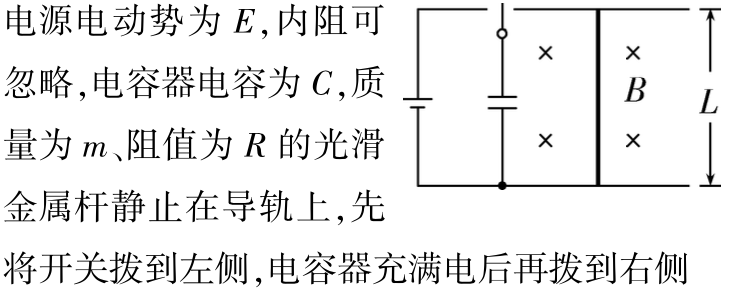
\includegraphics[width = \textwidth]{pictures/15.png}
        \caption*{Figure 1 情景}
    \end{minipage}
    \hfill
    \begin{minipage}{0.35\textwidth}
        \centering
        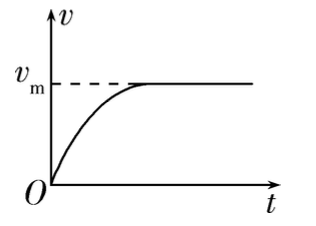
\includegraphics[width = \textwidth]{pictures/16.png}
        \caption*{Figure 2 运动过程}
    \end{minipage}
\end{figure}

\vspace{2em}

\begin{itemize}
    \item 能量角度:
          \vspace{5em}
    \item 动量角度:
          \vspace{5em}
    \item 习题

          \centering
          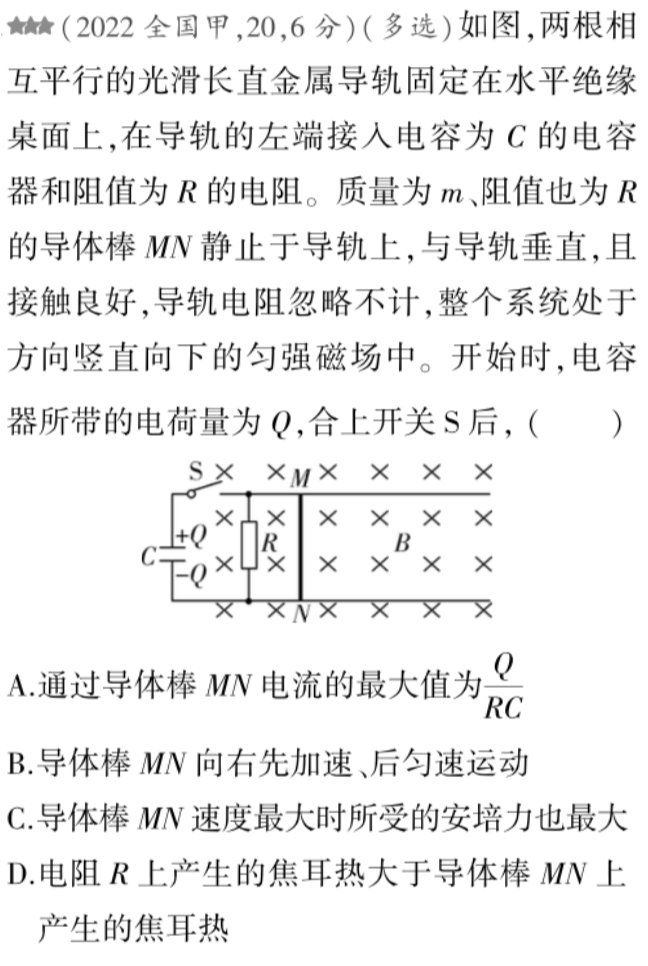
\includegraphics[width=0.45\textwidth]{pictures/20.png}
\end{itemize}


\end{document}